\begin{question}
\noindent Shape $A$ and shape $B$ are drawn on the coordinate grid below.

\begin{center}
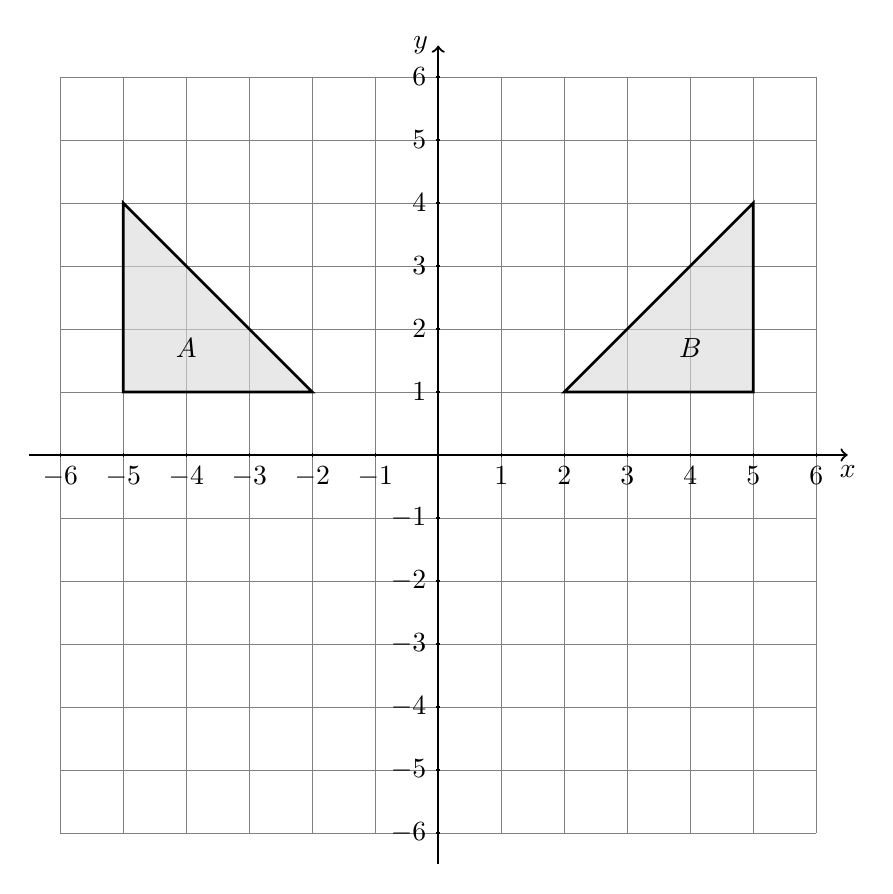
\begin{tikzpicture}[scale=0.8]
    \definecolor{borderColour}{HTML}{000000}
    \definecolor{fillColour}{HTML}{D8D8D8}

    \def\axisLimit{6}

    % Draw grid
    \draw[step=1cm,gray,very thin] (-\axisLimit,-\axisLimit) grid (\axisLimit,\axisLimit);

    % Draw axes
    \draw[thick,->] (-\axisLimit-0.5,0) -- (\axisLimit+0.5,0) node[anchor=north] {$x$};
    \draw[thick,->] (0,-\axisLimit-0.5) -- (0,\axisLimit+0.5) node[anchor=east] {$y$};

    % Label axes
    \foreach \x in {-6,-5,...,-1,1,2,...,6}
        \draw (\x cm,1pt) -- (\x cm,-1pt) node[anchor=north] {$\x$};
    \foreach \y in {-6,-5,...,-1,1,2,...,6}
        \draw (1pt,\y cm) -- (-1pt,\y cm) node[anchor=east] {$\y$};

    % Shape A: right-angled triangle with vertices (-5,1), (-5,4), (-2,1)
    \coordinate (A1) at (-5,1);
    \coordinate (A2) at (-5,4);
    \coordinate (A3) at (-2,1);
    \filldraw[fill=fillColour, draw=borderColour, line width=1pt, fill opacity=0.6] (A1) -- (A2) -- (A3) -- cycle;
    \node[left] at (A1) {};
    \node at (-4,1.7) {$A$};

    % Shape B: reflection of A in the y-axis: (5,1), (5,4), (2,1)
    \coordinate (B1) at (5,1);
    \coordinate (B2) at (5,4);
    \coordinate (B3) at (2,1);
    \filldraw[fill=fillColour, draw=borderColour, line width=1pt, fill opacity=0.6] (B1) -- (B2) -- (B3) -- cycle;
    \node at (4,1.7) {$B$};

\end{tikzpicture}
\end{center}

\noindent Describe fully the single transformation that maps shape $A$ onto shape $B$.

\vspace{4cm}
\answerlines{2}{2}
\end{question}
